% ---------------------------------------------------------------------------
% ElectroCom61 benchmark study
%
% DOCUMENT CLASS IS PROVISIONAL. `article` is a placeholder so the draft
% compiles anywhere; a venue template (IEEEtran, llncs, or whatever the target
% requires) will replace it later.
%
% Nothing outside this file should need to change when it does. The section
% files contain no preamble, no class-specific commands and no formatting
% assumptions -- only \section, \subsection, prose, and \ref/\citep. Tables and
% figures are pulled in from ../tables/ and ../figures/ by \input and
% \includegraphics, so switching class means editing the preamble below and
% nothing else.
%
% Two habits that keep that promise:
%   - reference tables and figures by \ref{}, never by a typed number;
%   - keep \graphicspath pointing at ../figures/ so figures are named by
%     filename alone and the path lives in exactly one place.
% ---------------------------------------------------------------------------
\documentclass[11pt,a4paper]{article}

\usepackage[utf8]{inputenc}
% lmodern MUST be loaded before fontenc, and both are load-bearing.
%
% T1 encoding alone switches Computer Modern to the EC fonts, which are
% distributed only as METAFONT sources. TeX then renders them as bitmaps, and
% the resulting PDF carries Type 3 fonts: text does not extract cleanly (the
% fi/ff ligatures come out as garbage, so "configuration" and "differs" break)
% and IEEE PDF eXpress rejects the file outright. Latin Modern is the same
% design as Computer Modern with the same T1 glyph coverage, but shipped as
% Type 1 outlines, so this one line makes the output scalable and searchable.
\usepackage{lmodern}
\usepackage[T1]{fontenc}
\usepackage[margin=1in]{geometry}

\usepackage{booktabs}     % \toprule, \midrule, \bottomrule -- all tables use these
\usepackage{graphicx}
\usepackage{natbib}
\usepackage{hyperref}
% NOTE: \Cref is NOT available -- cleveref.sty is not installed in this MiKTeX,
% and installing it is a network install. Cross-references use \ref with the
% type word typed ("Section~\ref{...}"), which is what Section 5 already does.
% No section, figure or table NUMBER is ever typed by hand.

\hypersetup{
  colorlinks=true,
  linkcolor=black,
  citecolor=black,
  urlcolor=blue,
}

% Figures are referenced by filename alone; the directory lives only here.
\graphicspath{{../figures/}}

% Figure width. Every figure in figures/ is RENDERED at 3.5 in -- one IEEE
% column -- with its font sizes chosen for that width. Including one at
% \columnwidth under this placeholder single-column article class scales it by
% 6.5/3.5, which took F1 from 8.95 in tall to about 16.6 in: taller than any
% page, so it could not be placed and floated past the bibliography.
%
% \figcol is the width figures are actually drawn at. Under a two-column venue
% template set it to \columnwidth instead -- there the rendered width and the
% column width agree, and every \includegraphics below follows automatically.
\newlength{\figcol}
\setlength{\figcol}{3.5in}

% Height cap. Width alone does not place these figures: F1 is 8.95 in tall at
% its design width, and this class gives a 9 in text block, so the figure plus
% its caption cannot fit on any page. LaTeX then defers the float to the end of
% the document, which is how both figures ended up after the bibliography.
%
% \figmaxh caps the height so figure and caption fit together on a float page.
% With keepaspectratio, whichever of the two limits binds first wins. Under a
% two-column venue template set \figmaxh to \textheight: there \figcol equals
% the real column width, the rendered size is already correct, and this cap
% never binds. It exists only to make the placeholder class able to show them.
\newlength{\figmaxh}
\setlength{\figmaxh}{0.86\textheight}

% Tables are generated into ../tables/ by scripts/make_tables.py and pulled in
% with \input{../tables/<name>}. They are never pasted into a section file.

\title{A Controlled Benchmark of Object Detectors on ElectroCom61}
\author{Diyar Walaa}
\date{\today}

\begin{document}
\maketitle

\begin{abstract}
% TODO: abstract. Write last.
\end{abstract}

\section{Introduction}
\label{sec:introduction}

% TODO: Motivate the study. The two prior papers on this dataset report
% contradictory results; say why a controlled benchmark is needed.

\section{Related Work}
\label{sec:related-work}

% TODO: Prior work on ElectroCom61, and on the detector families evaluated.

\section{Dataset Audit}
\label{sec:dataset-audit}

% Every number in this section traces to a committed run directory. Sources, by
% subsection:
%   3.1  runs/20260802_class_date_provenance/{class_split_counts.csv,
%        never_evaluated_classes.csv, summary.md}; data/master_results.csv
%   3.2  runs/20260802_class_date_provenance/date_split_summary.csv
%   3.3  runs/20260809_split_ratio_by_group_03/summary.md
%   3.4  runs/20260802_v1_provenance/summary.md;
%        runs/20260801_csv_coverage/split_agreement.csv
%   3.5  runs/20260809_split_v1_vs_v2_by_group_03/summary.md
%   3.6  runs/20260801_device_split/summary.md;
%        runs/20260809_split_v1_vs_v2_by_group_03/summary.md
%   3.7  runs/20260804_duplicate_contamination/summary.md;
%        runs/20260805_figure_verification_sheet_02/summary.md;
%        runs/20260802_burst_clusters_02/gap_histogram.csv
%
% THREE PLACES WHERE THE DRAFTED BULLET AND THE COMMITTED SOURCE DIVERGED. The
% source was followed in each case; see the report accompanying this draft.
%   3.3  the bullet said "within about one point" of 70/20/10. The run
%        classifies on IMAGES (within 1.5 images of a uniform draw) and states
%        explicitly that the percentage-point measure is the wrong one, because
%        it punishes a 54-image session for rounding it cannot avoid. At 1.0 pp
%        only THREE groups qualify, not four. Written on the images measure.
%   3.4  the bullet said T4 is decisive. The run designates T2 as the deciding
%        test and says so in bold: T1 can pass by arithmetic coincidence, so T4
%        rests on T2 having already established identity. Written that way.
%   3.5  the bullet said all eight v1 groups were near-nominal. The run scores
%        SEVEN of eight; the iPhone group misses the tolerance by 1.8 images
%        (0.95 pp) and the run flags it as near-nominal in substance but not by
%        the measure. Written as seven of eight with the borderline stated.
%
% PENDING CITATION -- 3.6. The dataset paper's stated rationale for using
% several phones ("to ensure diverse imaging qualities") cannot be cited:
% references.bib holds only yolov12paper and yolov13paper, with no entry for
% the ElectroCom61 dataset paper itself. The paragraph is written from the
% committed device measurement instead. Add the entry, then restore the
% rationale as a cited clause.

\subsection{Class coverage under the published split}
\label{sec:class-coverage}

The ten most-annotated classes in ElectroCom61, shown at the top of
Figure~\ref{fig:class-instance-counts}, hold at most two test instances each, and
eight of the ten hold none; the eleventh, IC-Base-14-Pin, holds 22.
The transition between the tenth and eleventh ranks is therefore a step rather
than a gradient. This is what distinguishes the pattern from class imbalance,
which is the reading the ordering first invites: an imbalanced dataset produces a
smooth decline in test representation as class frequency falls, and cannot
produce a discontinuity between adjacent ranks in which the more frequent side is
the empty one.

Fifteen of the 61 classes hold zero instances in both the validation and the test
partition, and 22 hold fewer than five test instances. A class with no test
instances cannot contribute to a test-set average precision at all, and a class
with one or two contributes a value estimated from a sample too small to
distinguish a detector from a coin.

Those fifteen classes, listed in Table~\ref{tab:unevaluable-classes}, are not
marginal. They carry 3{,}496 annotation instances between them, 27.0\% of the
12{,}937 in the dataset, and each holds between 153 and 293 training instances.
More than a quarter of the annotation effort in ElectroCom61 therefore supports
classes on which no published result has ever been measured.

The consequence is that every mAP figure reported on this dataset averages over
roughly 46 classes rather than 61, and the two averages are not comparable
quantities. The framework reports the count directly: under the published split
it evaluates 45 classes on validation and 46 on test, across all five detectors
trained here. A score computed over a reduced set of classes is not wrong, but it
answers a narrower question than its name suggests, which is why the count is
reported alongside every figure in Section~\ref{sec:results}.

\begin{figure}[t]
  \centering
  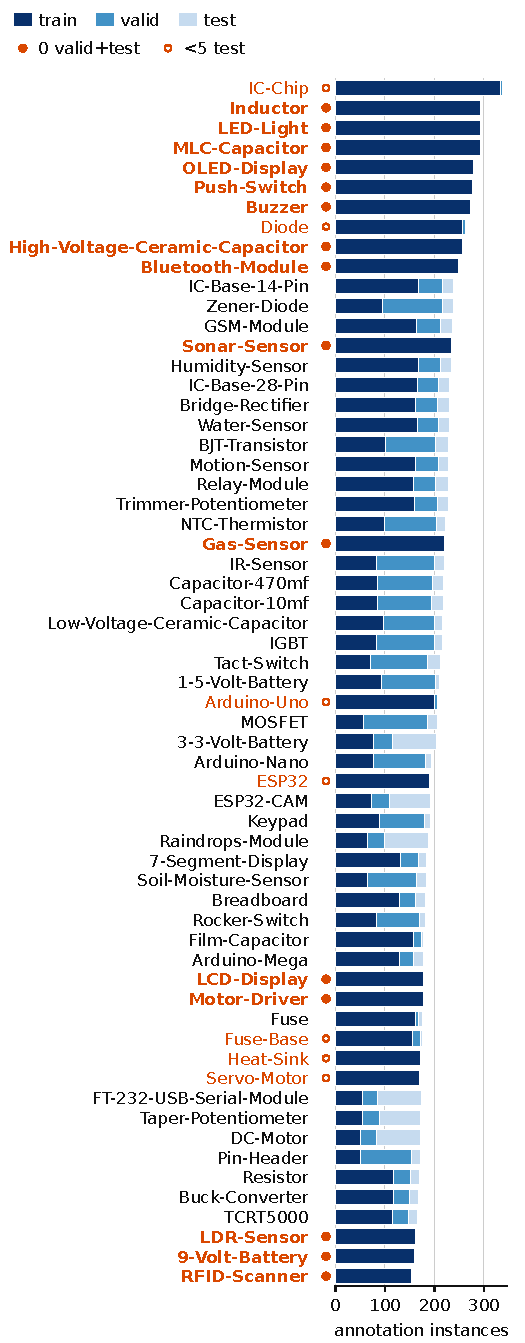
\includegraphics[width=\columnwidth]{f1_class_instance_counts.pdf}
  \caption{Per-class annotation counts, published split. 15 of 61 classes have
  zero valid+test instances (filled marker, bold label) and cannot be evaluated
  at all; 22 in total have fewer than five test instances --- the 15 above plus
  seven more, including IC-Chip, the most annotated class in the dataset.}
  \label{fig:class-instance-counts}
\end{figure}

% Generated by scripts/make_tables.py; carries its own \caption and \label.
\begin{table}[t]
  \centering
  \caption{The 15 classes with zero instances in both validation and test under the published split. Every instance of each sits in training, so none can be evaluated at all. Together they hold 3,496 of the dataset's 12,937 annotations, 27.0\%.}
  \label{tab:unevaluable-classes}
  \begin{tabular}{lrrr}
    \toprule
    Class & Train inst. & Train images & Total inst. \\
    \midrule
    Inductor & 293 & 188 & 293 \\
    LED-Light & 293 & 184 & 293 \\
    MLC-Capacitor & 292 & 81 & 292 \\
    OLED-Display & 279 & 189 & 279 \\
    Push-Switch & 277 & 177 & 277 \\
    Buzzer & 272 & 206 & 272 \\
    High-Voltage-Ceramic-Capacitor & 257 & 200 & 257 \\
    Bluetooth-Module & 249 & 179 & 249 \\
    Sonar-Sensor & 235 & 190 & 235 \\
    Gas-Sensor & 221 & 180 & 221 \\
    LCD-Display & 177 & 177 & 177 \\
    Motor-Driver & 177 & 175 & 177 \\
    LDR-Sensor & 161 & 79 & 161 \\
    9-Volt-Battery & 160 & 159 & 160 \\
    RFID-Scanner & 153 & 153 & 153 \\
    \midrule
    Total (15 classes) & 3,496 & 2,517 & 3,496 \\
    \bottomrule
  \end{tabular}
\end{table}


\subsection{The mechanism}
\label{sec:coverage-mechanism}

Three capture groups sit entirely within the training partition, as panel~(a) of
Figure~\ref{fig:capture-group-composition} shows: 19 February 2024, with 100
images; 20 February 2024, with 486; and the untimestamped iPhone group, with 189. Together they hold 775 images, 52.4\% of the 1{,}478 in the
training set, and none of the three contributes a single image to validation or
test.

All fifteen unevaluable classes occur only within those three groups. The
coverage gap in Section~\ref{sec:class-coverage} is therefore not a property of
the classes but of the sessions they were photographed in: a class that appears
only in a session allocated wholly to training cannot reach an evaluation
partition, however many instances of it the dataset contains. This is also what
makes the gap repairable, because it can be closed by reallocating sessions
rather than by collecting more data --- the construction taken up in
Section~\ref{sec:corrected-split}.

\begin{figure}[t]
  \centering
  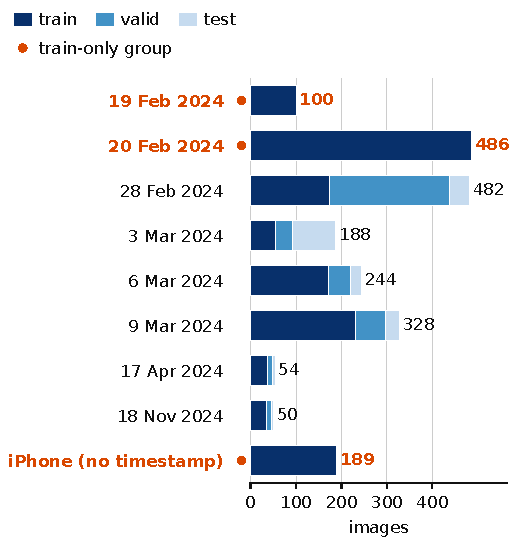
\includegraphics[width=\columnwidth]{f2_capture_group_composition.pdf}
  \caption{Capture-group composition of the published split. (a) v2 image counts
  per session: 3 of the 9 groups reach neither valid nor test (bold label, filled
  marker) and together hold 775 of the 1478 training images, 52.4\%; all 15
  classes that cannot be evaluated occur only within them. (b) the same sessions
  before and after the v2 re-split, each normalised to its own total, dashed
  lines where a 70/20/10 split would fall.}
  \label{fig:capture-group-composition}
\end{figure}

\subsection{Allocation is not uniform across sessions}
\label{sec:allocation-uniformity}

Measured session by session, the split takes three distinct shapes. Four groups
--- 6 March, 9 March, 17 April and 18 November 2024 --- fall within 1.5 images of
what a uniform 70/20/10 draw over that group would have produced, which is as
close as integer arithmetic permits. Three contain no validation or test images
at all. The remaining two are strongly skewed in opposite directions: 28 February
2024 holds more validation images than training images, at 35.9/55.2/8.9, and 3
March 2024 holds more test images than training images, at 29.3/20.2/50.5. The
tolerance is expressed in images rather than percentage points because a
54-image session moves 1.9 points per file, so a points-based tolerance would
score it as skewed for rounding it cannot avoid.

Aggregated over all 2{,}121 images the split is 69.7/20.7/9.7, which reads as a
textbook 70/20/10. That aggregate is an accident of offsetting deviations.
Relative to a uniform draw, the three train-only groups withhold 155.0
validation images and 77.5 test images between them; the 28 February group
carries a validation surplus of 169.6 and the 3 March group a test surplus of
76.2. The two nearly cancel, leaving the aggregate 13.8 validation images above
and 7.1 test images below nominal --- under one percentage point in each case.
This is why the problem is invisible at the level at which splits are normally
checked, and it is the reason the per-group measurement was made at all.

\subsection{The metadata file describes v1, not v2}
\label{sec:metadata-provenance}

The metadata CSV shipped inside the v2 archive was tested against an actual v1
download under four provenance tests, and passed all four. The deciding test is
the identity test: the set of image stems in v1 and the set of keys in the CSV
are equal, with zero entries on either side unmatched. Identity is what settles
the question, because the count test can pass by arithmetic coincidence --- two
collections of 2{,}071 files need not be the same files. With identity
established, the split-level test is decisive in turn: the CSV's
\texttt{DATA\_TYPE} column against the folder each image occupies under v1 gives
a perfectly diagonal contingency table, 1{,}454 train, 412 validation and 205
test, with zero disagreements across all 2{,}071 rows.

An independent line of evidence corroborates this. Fifty images in v2 carry no
CSV row at all, and those fifty are split 35/10/5 across train, validation and
test. That is exactly the composition of the 18 November 2024 capture session,
which is the one session absent from v1 entirely. The images the CSV does not
describe are precisely the images that did not exist when it was written.

The consequence is a rule for reading the dataset rather than a defect in it. The
folders on disk are authoritative for the v2 split and the CSV is not: the same
contingency table built against v2 carries 600 off-diagonal rows. But the CSV
remains a faithful record of the v1 assignments, and it is the only surviving
record of them, which is what makes the comparison in the next subsection
possible.

\subsection{What the v2 re-split changed}
\label{sec:v2-resplit}

Under v1, seven of the eight capture groups the CSV covers were near-nominal by
the same 1.5-image measure used above. The eighth, the untimestamped iPhone
group, misses that tolerance by 1.8 images on a 189-image group --- 0.95
percentage points --- so the departure from a uniform draw is a rounding-scale
one in every group present.

The v2 re-split, drawn in panel~(b) of
Figure~\ref{fig:capture-group-composition}, left three of those groups untouched,
with zero images moved in 6 March, 9 March and 17 April, and changed the other
five. In the three groups that
became train-only, validation and test images were folded into training: 20
validation and 10 test images for 19 February, 97 and 48 for 20 February, and 36
and 20 for the iPhone group. The two skewed groups absorbed the resulting
deficits, with 28 February taking the validation shortfall through 189 images
moved from training to validation, and 3 March taking the test shortfall through
77 moved from training to test.

Across the 2{,}071 images the CSV covers, 600 changed assignment between v1 and
v2 --- 29\% of them. These are the same 600 images that produce the off-diagonal
rows in the \texttt{DATA\_TYPE} comparison of
Section~\ref{sec:metadata-provenance}; the disagreement between the CSV and the
folders is a record of the re-split, not an inconsistency within either.

One further observation constrains what can be inferred from the above. The 18
November 2024 session, which was added in v2 and has no v1 assignment to change,
was split 35/10/5 of 50 --- exactly 70/20/10, with zero deviation in any of the
three cells. Whatever produced the v2 split allocated a new session at the
nominal ratio. No mechanism is claimed here for the changes to the pre-existing
assignments; the observation is recorded because it bounds the explanations that
remain available.

\subsection{One camera is never evaluated}
\label{sec:camera-coverage}

Under v1, the 189 untimestamped images, which the metadata attributes to an
iPhone, were split 133\slash 36\slash 20 across train, validation and test. Under
v2 they are split 189\slash 0\slash 0, so every image from that device now sits
in the training partition.

The dataset records four distinct device names across its 2{,}121 images, and the
iPhone is the only one confined to a single partition. Whatever variation in
imaging characteristics that device contributes --- sensor, optics, and the
processing pipeline applied before the image was ever exported --- is therefore
present in what the detectors learn from and absent from what they are measured
on. A model that generalises poorly to that device would not register as
degraded under the published split, because no test image would expose it.

% TODO: the dataset paper states that several phones were used to ensure diverse
% imaging qualities, which is the sentence that makes this subsection's
% implication sharp. It cannot be cited until references.bib carries an entry
% for the dataset paper. Restore as a cited clause once it does.

\subsection{Duplicate contamination: a negative result}
\label{sec:duplicate-contamination}

The published split carries no test--train near-duplicate pairs at any threshold
tested, under either of the two scorings applied, with low-information pairs
excluded. This is reported as a finding rather than as an absence of one. The
split has a documented coverage defect, established above, and the natural
suspicion is that a split allocated in a way that stranded three whole sessions
in training might also have scattered near-identical frames across the boundary.
It did not, and a corrected split must therefore preserve this property rather
than merely avoid making it worse.

The margin behind that result is thin and is disclosed here rather than left to
be discovered. The closest test--train pair scores 0.0515 against the loosest
threshold applied, 0.05, clearing it by 3\%. A threshold chosen slightly more
conservatively would have returned a non-zero count, so the result is
threshold-sensitive and should be quoted with the threshold attached.

No threshold can be derived empirically from the data itself. The distribution of
gaps between consecutive captures is unimodal: measured per second of bin width,
it rises monotonically to a peak in the 3--5 second bin and decays monotonically
thereafter, on both of the two independent device keyings tested. There is no
valley between a burst mode and a between-burst mode at which a cut could be
placed, because there is only one mode. Any grouping threshold is consequently a
construction rather than a measurement, which is why the one adopted in
Section~\ref{sec:corrected-split} is justified by the properties of the split it
produces rather than by the shape of this distribution.

Two scope limits travel with every figure above. Only pairs sharing an identical
class inventory are compared, so a genuine duplicate in which one component is
occluded in one frame is never scored; every count is a floor rather than an
estimate. And 95 low-information cross-split pairs, those carrying two annotated
boxes or fewer, are excluded from the ranking, because a match between box
centres is cheap to achieve by chance when there are few boxes to match.

\section{A Corrected Split}
\label{sec:corrected-split}

% Every number in this section traces to a committed run directory. Sources, by
% subsection:
%   4.1  runs/20260804_burst_aware_split_04/summary.md; tables/t2_split_properties
%   4.2  runs/20260801_device_split/summary.md (filename taxonomy);
%        runs/20260804_burst_aware_split_04/config.json (tau, seed, eps)
%   4.3  runs/20260804_burst_aware_split_04/{summary.md, groups_moved.csv,
%        moves.csv}; tables/t2_split_properties (39 of 61 -> 61 of 61)
%   4.4  runs/20260804_burst_aware_tau_sweep/summary.md
%   4.5  runs/20260803_corrected_split_02/summary.md (image-level allocator);
%        runs/20260804_burst_aware_split_03 via the sweep row at tau=30;
%        runs/20260814_figure_near_duplicate/per_box_centre_shift.csv
%   4.6  runs/20260804_build_corrected_dataset_02/summary.md
%   4.7  runs/20260804_duplicate_contamination/summary.md;
%        runs/20260805_consecutive_counter_pairs/
%   4.8  README.md licence section; data/kaggle/latency_history/pass2.json
%
% UNSUPPORTED BULLET, LEFT AS A TODO RATHER THAN WRITTEN. See 4.6 below: the
% drafted bullet claimed 364 same-camera cross-split pairs within 15 s in both
% the published and the corrected split. No committed run reports that figure.
% The nearest committed measurements are different quantities and must not be
% substituted for it:
%   - runs/20260803_corrected_split_02/ reports cross-split adjacent pairs
%     537 before / 600 after, but for the SUPERSEDED image-level allocator, not
%     the released one, and over all gaps rather than a 15 s window.
%   - runs/20260804_burst_aware_split_04/ reports 177 groups already straddling
%     the boundary before any move, which counts groups, not pairs.
% Producing the claimed figure needs a script and a run directory of its own.
%
% F3 LEGIBILITY -- MEASURED, NOT ESTIMATED. near_duplicate_pair is rendered at
% 11.0 x 7.4 in and its smallest text (the per-box shift table) is 6.9 pt at
% that size. Included at \figcol (3.5 in) that text renders at 2.2 pt; at
% \textwidth (6.5 in) at 4.1 pt. Both are below the 8 pt floor every other
% figure in this paper is built to. It is included below at \textwidth because
% that is the least bad option available, and it needs a re-render at target
% width before submission. Scaling cannot fix it.

The audit of Section~\ref{sec:dataset-audit} establishes a defect that is
repairable without collecting data: fifteen classes are unevaluable because the
sessions containing them were allocated wholly to training. This section
constructs a split that repairs it, states the constraints the repair had to
satisfy, and reports what it does and does not achieve. The construction is
released as a manifest rather than as a claim.

\subsection{What a correction has to satisfy}
\label{sec:correction-constraints}

Four constraints define the problem. Every class must reach at least five
instances in both the validation and the test partition, which is what makes it
evaluable at all. The split sizes must stay exactly 1478/438/205. No image may
be added, removed or modified. And test--train near-duplicate contamination,
which Section~\ref{sec:duplicate-contamination} measured at zero, must not
increase. The first is the objective; the other three are the price of a
correction that can be compared against the split it replaces.

The size constraint is the one that most needs defending, because it is the one
that costs the most. If the corrected training set were larger or smaller than
the published one, any later difference in accuracy between the two could be
attributed to the amount of training data rather than to its composition, and
the comparison in Section~\ref{sec:results} would answer a question nobody
asked. Freezing the three counts exactly means the only difference between the
two experiments is which images sit in which partition. It also makes the
correction harder: every image admitted into validation or test must be paid for
by another image returned to training.

\subsection{The grouping rule}
\label{sec:grouping-rule}

Whole capture bursts move as a unit; individual images never move alone.
Section~\ref{sec:duplicate-contamination} established that burst structure
exists in this dataset, and a burst is precisely a set of frames showing the
same scene seconds apart. Moving one frame out of a burst therefore places a
near-duplicate of a training image into an evaluation partition, which is the
contamination the fourth constraint forbids. Making the burst the atomic unit
of movement rules that out by construction rather than by detection: a group
that cannot be split cannot straddle the boundary.

Bursts are formed at a 15-second gap threshold and, critically, per camera
rather than globally. Sorting every image in the dataset by timestamp and
cutting at gaps would interleave frames from two photographers shooting at the
same moment on different devices, manufacturing groups that never existed as
capture events. Clustering within each device first and only then applying the
gap threshold keeps a group a record of one camera's continuous activity.

The grouping rule needs a taxonomy of filenames because the archive does not
carry one. Three families encode a timestamp and can be clustered in time; a
fourth cannot. Nine images carry an additional \texttt{\_NN} sub-index
appended to their timestamp, which resolves frames sharing a capture second.
The 189 untimestamped images admit no temporal clustering at all, so for those
the grouping falls back to scene content --- matching class inventory and box
geometry --- which groups by appearance rather than by time. That substitution
is weaker than a burst and is recorded as such: it is an inference about which
photographs show the same arrangement, not a measurement of when they were
taken.

\subsection{The allocation}
\label{sec:allocation}

The allocator begins from a per-class deficit: for each of the 61 classes, how
many further instances validation and test each need to reach five. Under the
published split 39 of the 61 classes already clear that bar in both partitions,
so 22 carry a deficit, and 15 of those 22 carry the maximum possible one, having
no instances in either partition to begin with.

Groups are then selected greedily, each step taking the group that closes the
largest number of outstanding deficits at once. This is why the repair is so
much cheaper than the deficit count suggests: a single capture group contains
several components photographed together, so admitting one group can lift
several classes over the bar simultaneously. Across the whole allocation 68
images move, and they repair all 22 classes --- taking the split from 39 of 61
to 61 of 61, as Table~\ref{tab:split-properties} records.

An equal number of images is returned to training, which is what holds the sizes
exactly. Only groups lying wholly inside one partition are eligible to be
returned, because returning part of a group would reintroduce the straddling
that Section~\ref{sec:grouping-rule} exists to prevent, and a group may be
returned only if removing it leaves every class still at or above five. The
dataset divides into 776 atomic groups, of which 177 already straddle a
partition boundary in the published split and are left untouched. Of the
remainder, validation admitted 18 groups and returned 10; test admitted 13 and
returned 6.

\subsection{Why 15 seconds}
\label{sec:tau-choice}

Class feasibility never bound the choice of threshold. At every value swept ---
15, 20, 25, 30, 35, 45 and 60 seconds --- all fifteen rescued classes retain two
or more qualifying groups, so the criterion the threshold was originally
introduced to satisfy is satisfied everywhere. Panel~(b) of
Figure~\ref{fig:tau-sweep} shows that row filled across the entire sweep, which
is the negative result that makes the rest of this subsection necessary: had
feasibility bound, the choice would have been made for us.

What bound it was the return budget. As the threshold grows, groups grow, and
the number of images the test partition can safely give back collapses --- 59 at
15 seconds, 26 at 25, 10 at 30, and 1 at 60 --- while the number it owes rises
in the opposite direction, from 15 to 31. The two cross between 25 and 30
seconds, and past that crossing the split cannot be rebalanced at all: at 30
seconds test owes 20 images and can return only 10, so the sizes end at
1458/438/225.

Fifteen seconds is the smallest value satisfying both constraints, and among the
three values that hold the sizes it moves the fewest images: 68, against 78 at
20 seconds and 80 at 25. It is not the value that moves the fewest images
overall. Thirty seconds moves 64, four fewer, and is excluded because it breaks
the sizes rather than because it is more expensive.

The criteria do not fail monotonically, and reporting only the chosen value
would hide that. Forty-five seconds is clean on contamination --- zero
test--train pairs at every epsilon under both scorings --- yet fails on sizes,
ending at 1448/438/235. Thirty-five and 60 seconds each carry one test--train
pair at $\epsilon = 0.05$ under aligned scoring, while both are clean under raw
scoring at the same threshold, which is why the scoring must be named whenever
that column is quoted. A threshold chosen by scanning upward until the first
failure would have stopped at the wrong place.

\begin{figure}[tp]
  \centering
  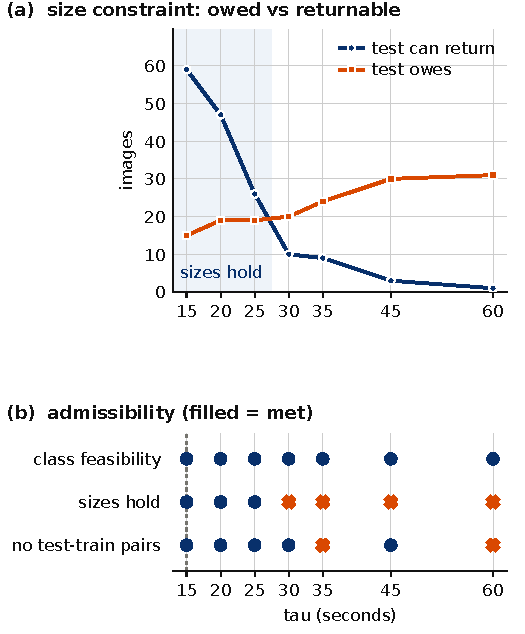
\includegraphics[width=\figcol,height=\figmaxh,keepaspectratio]{f4_tau_sweep.pdf}
  \caption{Why the released split uses $\tau = 15$~s. (a) the size constraint:
  at each $\tau$, the images the test split owes back after admitting whole
  groups, against the images it can safely return. The two cross between 25 and
  30~s, and past that point the split cannot be rebalanced --- at $\tau = 30$~s
  test owes 20 and can return only 10, ending at 1458/438/225 instead of
  1478/438/205. (b) the three admissibility criteria. Class feasibility is
  satisfied at every $\tau$ tested, so it never bound the choice; what bound it
  was the collapsing return budget in (a). $\tau = 15$~s is the smallest value
  meeting all three.}
  \label{fig:tau-sweep}
\end{figure}

\subsection{How the split was arrived at}
\label{sec:split-iterations}

The released split is the third of three attempts, and the two it replaced are
reported here rather than discarded. The sequence is evidence that the
constraints in Section~\ref{sec:correction-constraints} were binding on the
construction rather than assembled afterwards to describe whatever the final
allocator happened to produce.

The first attempt moved individual images. It succeeded on the objective and on
the sizes: 64 images moved, all 61 classes cleared the bar, and the split ended
at 1478/438/205 exactly. It failed on contamination, and the failure is
concrete. It moved \texttt{IMG\_20240220\_115315} into test while
\texttt{IMG\_20240220\_115316} --- captured one second later, showing the same
five components --- stayed in training. Across those five components the box
centres differ by at most 9.01 pixels on a 640-pixel canvas. That single
decision created 2 test--train near-duplicate pairs under raw scoring and 4
under aligned at $\epsilon = 0.05$, where the published split had none, which is
what established that an allocator blind to duplicates can satisfy every other
constraint and still make the split worse.

The second attempt made whole groups the unit of movement at a 30-second
threshold. It eliminated the contamination --- zero test--train pairs at every
epsilon under both scorings --- and broke the sizes instead, ending at
1458/438/225. Having each constraint satisfiable alone, and the two attempts
failing on different ones, is what motivated sweeping the threshold rather than
choosing it.

The third attempt swept the threshold across seven values and found that 15, 20
and 25 seconds all satisfy both constraints, of which 15 is the smallest and the
cheapest. That is the released split: $\tau = 15$~s, scene threshold
$\epsilon = 0.05$, seed 20260804.

Both superseded runs are retained in the repository with a banner recording why
they were replaced, and no number inside either was altered when they were
superseded. A run whose conclusion was overturned is still the only record of
what was actually computed at the time, and editing it would destroy the
evidence that the sequence above took place.

% F3 at \textwidth, not \figcol: see the legibility note in this file's header.
% This is a wide two-panel exhibit; even \textwidth leaves its shift table at
% 4.1 pt. It needs a re-render at target width before submission.
\begin{figure}[tp]
  \centering
  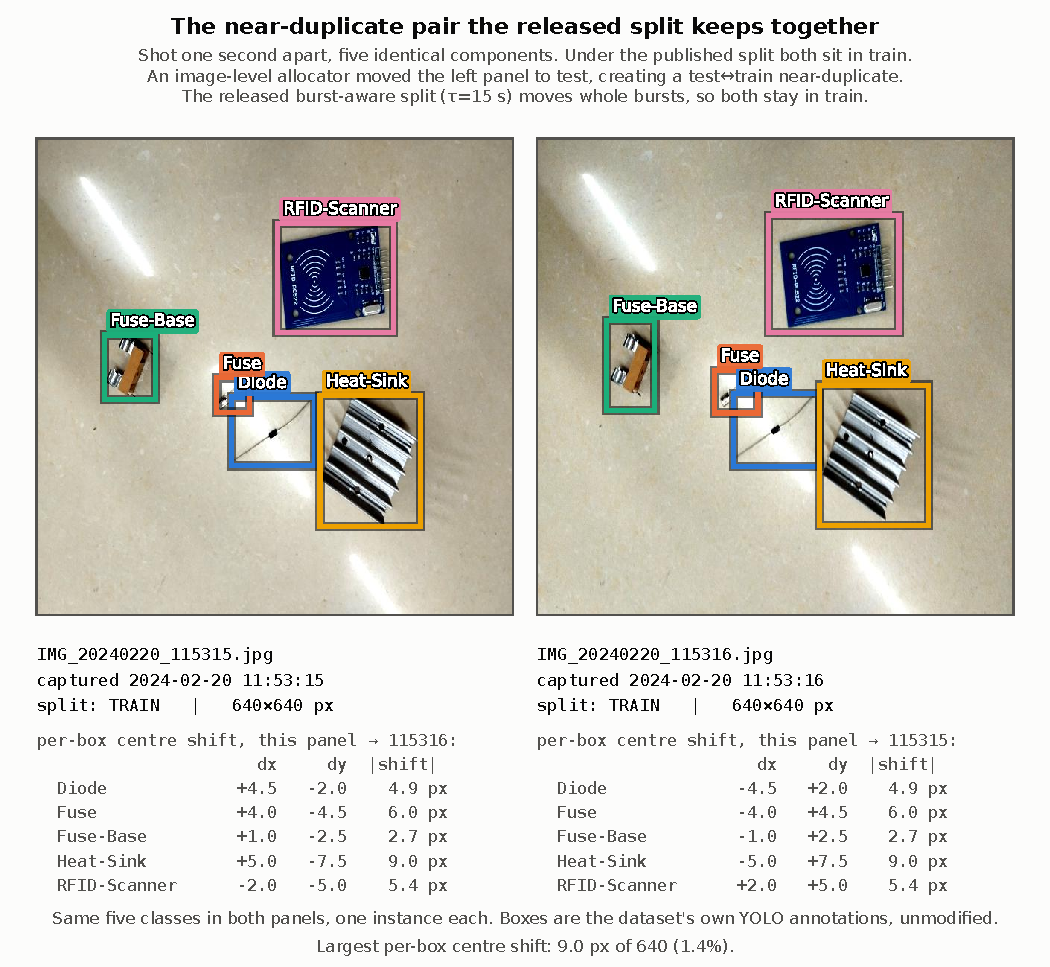
\includegraphics[width=\textwidth]{near_duplicate_pair.pdf}
  \caption{The pair that decided the grouping rule.
  \texttt{IMG\_20240220\_115315} and \texttt{IMG\_20240220\_115316}, captured
  one second apart, with their annotation boxes drawn and named. Across the five
  shared components the box centres differ by at most 9.01 pixels on the
  640-pixel canvas. The first allocator placed the left frame in test and left
  the right in training; the released split moves whole bursts, so both sit in
  training. The split shown under each panel is read from the built tree, not
  asserted, so the figure tracks whatever split is released.}
  \label{fig:near-duplicate-pair}
\end{figure}

\subsection{Verification}
\label{sec:split-verification}

The corrected dataset was materialised by copying from an unmodified v2 tree and
then verified by re-reading what had been written, under eight checks, all of
which pass. The image counts per partition are 1478/438/205; the copy loop's
intent matches what is on disk; no image lacks a label and no label is an
orphan; the total instance count is 12{,}937, unchanged; all 61 classes hold at
least five instances in both validation and test; every class identifier lies in
the range 0 to 60; and every copied file is byte-identical to its source.

The byte-identical check earns its place precisely because it is redundant with
the others under normal conditions. A truncated or partially written copy would
pass every count-based check in the list --- the file exists, it has a label, the
label parses, the class identifiers are in range --- while silently corrupting
the pixels a detector trains on. Comparing content hashes across all 2{,}121
images and their 2{,}121 label files is the only check in the set that would
catch it.

% TODO -- UNSUPPORTED, DO NOT WRITE UNTIL A RUN EXISTS. The drafted bullet here
% reported an independent check on the allocator: same-camera cross-split pairs
% within 15 s numbering 364 in the published split and 364 in the corrected one,
% showing the allocator neither created nor removed any. No committed run
% reports that figure, and the nearest committed numbers measure different
% things (see this file's header). The claim is worth making -- it is a check on
% temporal adjacency independent of the label-geometry contamination measure --
% but it needs a script and its own run directory first.

\begin{table}[t]
  \centering
  \caption{Properties of the published split and of the corrected split released here. Near-duplicate pair counts are at $\epsilon = 0.05$ with low-information pairs excluded, reported separately for raw and aligned scoring. The corrected split holds the image counts of the published one exactly, so no accuracy difference can be attributed to training-set size.}
  \label{tab:split-properties}
  \begin{tabular}{lrr}
    \toprule
    Property & Published & Corrected \\
    \midrule
    Images (train / val / test) & 1,478 / 438 / 205 & 1,478 / 438 / 205 \\
    Classes with $\geq$5 inst. in val and test & 39 of 61 & 61 of 61 \\
    Classes with zero val+test instances & 15 & 0 \\
    test$\leftrightarrow$train pairs (raw / aligned) & 0 / 0 & 0 / 0 \\
    val$\leftrightarrow$train pairs (raw / aligned) & 1 / 3 & 1 / 3 \\
    val$\leftrightarrow$test pairs (raw / aligned) & 0 / 0 & 0 / 0 \\
    Images reassigned & --- & 68 \\
    Grouping $\tau$ (s) & --- & 15 \\
    Seed & --- & 20260804 \\
    \bottomrule
  \end{tabular}
\end{table}


\subsection{What the correction does not fix}
\label{sec:correction-limits}

Validation--train contamination is unchanged. At $\epsilon = 0.05$ the published
split and the corrected one both carry 1 such pair under raw scoring and 3 under
aligned, and they are the same pairs: pre-existing in the data as distributed,
created by neither allocator and removed by neither. The zero reported in
Section~\ref{sec:duplicate-contamination} and preserved here describes the
test--train relationship only. Test contamination biases the headline metric and
validation contamination biases model selection; they are different failures and
a single cross-split figure that merged them would report neither.

The rescued classes rest on very few images each. Five instances is the
threshold at which a class becomes measurable, not the sample size at which a
per-class average precision becomes worth quoting with confidence. The
correction changes those classes from unmeasurable to measurable and claims
nothing beyond that, and per-class results in Section~\ref{sec:results} should be
read with the instance count beside them.

The duplicate measurement's scope carries over unchanged from
Section~\ref{sec:duplicate-contamination}: only pairs sharing an identical class
inventory are ever compared. Among the untimestamped images, three
consecutive-numbered pairs fall outside that scope, one of them across train and
test. \texttt{IMG\_5243} carries six classes to \texttt{IMG\_5244}'s five, the
extra being an Arduino-Uno, and the two shared single-instance components sit
109.6 and 86.3 pixels apart on the 640-pixel canvas. Inspected visually, the
scene is rearranged rather than re-photographed. That pair was never scored, and
never scored is not the same as scored and cleared.

Partial overlap between images is pervasive and no split removes it. Every image
in a capture session shares a background and draws from the same pool of
components, so a training image resembling a test image in background and in
several components is the normal condition of this dataset rather than a defect
of any particular allocation. The contamination figures are bounded claims about
identically inventoried pairs, and they are not a guarantee that no training
image resembles a test image.

The threshold is established for one seed. The allocator is greedy, and a
different seed explores a different corner of the search space; the sweep in
Section~\ref{sec:tau-choice} answers the question for seed 20260804 and does not
prove that 15 seconds is the right threshold in general. What it establishes is
that a threshold satisfying every constraint exists and that this one does.

\subsection{What is released}
\label{sec:split-release}

The split is released as a manifest assigning each image name to a partition.
Applied to a copy of ElectroCom61 v2 obtained from the Mendeley archive, it
reproduces the corrected split exactly, because the seed is fixed and the
allocation deterministic. The manifest is offered under CC BY 4.0, the licence
of the dataset it derives from, and the attribution to the dataset authors
travels with it \citep{electrocom61}.

A copy of the re-split images is also published alongside the manifest, as a
convenience for anyone who would otherwise download the archive and rebuild the
tree locally. That copy is a redistribution of the dataset's images, carries the
same CC BY 4.0 terms and the same attribution, and modifies nothing: the
corrected split changes which directory an image sits in and no image's pixels
or annotations. Both artefacts describe the same assignment, and the manifest is
the authoritative one --- it is what the verification in
Section~\ref{sec:split-verification} was run against.

\section{Benchmark Setup}
\label{sec:benchmark-setup}

% TODO: 5.1 and 5.2 are drafted below. Still to write: 5.3 (the RT-DETR
% learning-rate deviation), and the evaluation protocol.

\section{Results}
\label{sec:results}

% TODO: Accuracy and efficiency. Tables t4_main_results, t5_efficiency,
% t6_latency_breakdown. Figures f5_published_vs_corrected,
% f6_accuracy_vs_latency.

\section{Discussion}
\label{sec:discussion}

% TODO: Interpretation. Includes the framework-version argument and the
% two prior-work findings recorded in notes/writing-corrections.md.

\section{Limitations}
\label{sec:limitations}

% TODO: Single seed, one GPU, no variance estimate. The augmentation
% confound. The scope limit on the contamination figures.

\section{Conclusion}
\label{sec:conclusion}

% CONSTRAINTS THIS SECTION IS HELD TO, since a conclusion is where they slip:
%   - No number appears here that does not appear earlier. The figures used are
%     15 of 61, the ten most-annotated classes, five detectors, and the 45/46
%     evaluated-class counts, all from Sections 3 and 5.
%   - The 45 and 46 in the opening sentence MUST keep their "computed on the
%     published split" scoping. Unscoped they read as properties of the dataset
%     rather than of the partition, which is the error the whole paper is about.
%     The same scoping is carried at every other site: 3.1, 5.4, 7.1 and 7.2.
%   - No citation. Every sentence here restates something this paper
%     established, so a citation would either be redundant or would smuggle in a
%     claim the body has not made.
%   - No verbatim overlap with Section 7. Checked mechanically, the same way
%     Section 2 was: no sentence over 60 characters is shared between them.
%
% THE FIRST PARAGRAPH CARRIES THE DEVIATION, CHANGED 2026-08-15. It read "under
% a single configuration" and then "the benchmark holds every setting but the
% architecture fixed" -- two flattenings of 5.3 in consecutive sentences, the
% second flatly contradicted by it. RT-DETR-l needs a learning rate a
% hundredfold lower and does not train at all without it. Both now carry the
% exception, and "otherwise" is load-bearing in the second. Matched to 5.2's own
% wording and to the same edit in the abstract and Section 1's contribution 3.
%
% THE LAST PARAGRAPH DEPENDS ON SECTION 10. "released as a manifest, with the
% scripts and run records" has somewhere to point only because
% sections/10-availability.tex names a repository and an archived identifier.
% That DOI is a PLACEHOLDER as of 2026-08-15; if it is never minted, this
% paragraph and the abstract's closing sentence both need softening.
%
% The paragraph most at risk is the fourth. Section 7.2 lists three checks that
% would have CAUGHT the defect; this lists four things a study can REPORT. The
% overlap is real and deliberate -- they are the same underlying quantities --
% so the wording is kept deliberately distinct, and the framing is prospective
% rather than retrospective.

A detection result reported on ElectroCom61 measures less than its name suggests:
computed on the published split it averages over 45 classes on validation and 46
on test rather than 61, reported as a bare mAP@50 it rests on the metric whose
ranking moves when the split changes, and reported without a timing measurement
it cannot say whether the model is fast enough for the conveyor the dataset was
assembled for.

This paper audited ElectroCom61 from its released files alone, constructed and
released a corrected split, and trained five detectors on both the published and
the corrected partition under one configuration, with a single documented
deviation: the transformer detector will not train at the learning rate the four
convolutional ones are trained at. The audit needed no model and no pixels; the
benchmark otherwise holds every setting but the architecture fixed, so that
differences between the two splits are attributable to the split.

The audit found that the published partition cannot evaluate 15 of the 61
classes at all, because they hold no instances in either the validation or the
test set. The cause is how capture sessions were allocated rather than how rare
those classes are. Rarity would leave the least frequent classes unevaluable and
no others; instead the fifteen span almost the entire frequency range, and eight
of the ten most heavily annotated classes are among them.

The benchmark found that correcting the split raises every model's score, on
both accuracy metrics and both evaluation partitions, without exception. The
defect had been understating measured performance rather than overstating it,
because what it withheld from evaluation was easier than what it left in. That
is the reverse of what a defective split is normally expected to do, and it is
the reason such a defect is easy to leave in place: a result that is too low
attracts no scrutiny.

Four things could be reported at no cost by any study on any dataset, and each
would have exposed something the record for this one does not show. How many
classes the metric was actually computed over, which the framework prints
without being asked. How each capture session was divided, not only the totals
across the dataset. Which version of the data, which partition and which seed
produced a figure. And a timing measurement, without which an accuracy ranking
cannot say whether the better model is fast enough to use.

The corrected split is released as a manifest, with the scripts and run records
that produced and verified it, so that every figure reported here can be
recomputed rather than taken on trust. What this study cannot establish from one
dataset is how often the defect it describes occurs elsewhere; establishing that
would take the checks above, which cost minutes each, run against other
benchmarks whose collection was organised in sessions.


\bibliographystyle{plainnat}
\bibliography{references}

\end{document}
